\section{Introduction and contributions}\label{sec:intro}
We study the dynamics on the positive integers in which a state $m$ moves to
\[
 T_N(m)=m\,R(N),\qquad R(N)=\frac{(N+1)^2}{N},
\]
whenever the \emph{label} $N\ge1$ divides $m$. In the UNNS programme this is the integer grammar SELECT-II~\cite{FoundI,RefColl}; Manuscript~I~\cite{PaperI} studied the geometry carried by a single state of the programme's arithmetic, and the present manuscript studies what happens \emph{between} states. A finite sequence of such moves is a \emph{history}. The point of view taken here is that the history is a mathematical object in its own right: it has an arithmetic (which words of labels are admissible from which sources), a combinatorics (how many histories end at one integer, how adjacent exchanges connect them) and a topology (cell complexes whose vertices are histories), and none of this is recoverable from the integer at which a history ends.

\paragraph{The four histories of $72$.}
The integer $72$ is reached from four complete histories (\cref{fig:objects}, \cref{fig:four}):
\[
 1\to4\to16\to72,\qquad 1\to4\to18\to72,\qquad 3\to16\to72,\qquad 10\to72 .
\]
The first two have the same source, content $\{1,1,2\}$ and endpoint, and differ by one exchange of adjacent labels; the third and fourth have other contents altogether. The same endpoint hides three contents and three swap classes. The contribution of this manuscript is to show that this phenomenon is governed by exact arithmetic that can be stated and proved, and to chart the topology it produces.

\begin{figure}[tbp]\centering
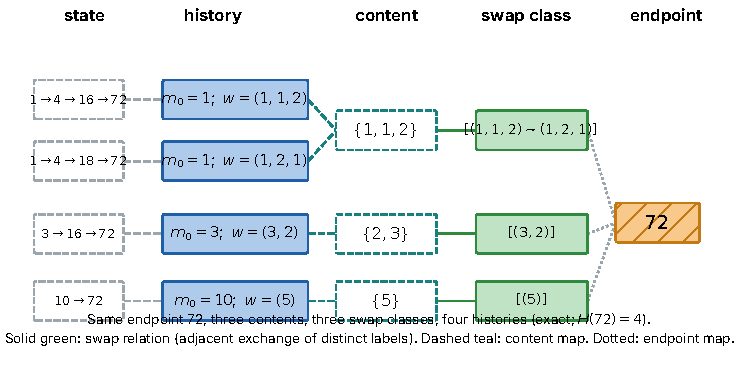
\includegraphics[width=\textwidth]{fig01_objects}
\caption{\textbf{Objects and equivalence relations (exact, endpoint $72$).} The four complete histories ending at $72$ (middle left, with their state sequences in dashed boxes), their three contents, the swap classes they fall into, and the common endpoint. Source $m_0$ and word $w$ are as in \cref{def:history}; the swap relation is \cref{def:swapgraph}.}\label{fig:objects}
\end{figure}

\paragraph{Contributions.}
The results are organised in nine groups, HII-1 to HII-9; each is a part of the programme's allocation for Manuscript~II and is tagged in the text by the identifiers of the source records it restates (\cref{app:crosswalk}).
\begin{enumerate}[leftmargin=2.2em,itemsep=2pt]
\item[\textbf{HII-1}] \emph{Complete ancestry and counting} (\cref{sec:ancestry}). The predecessors of an integer $t$ correspond to the squares $d^2\mid t$; $H(t)=\sum_{d^2\mid t}H(t(d-1)/d^2)$ with $H=1$ on squarefree $t$, and the recursion terminates because $R(N)\ge4$ (\cref{thm:predecessors}). $H(72)=4$, $H(72^r)\ge\binom{2r}{r}$ (\cref{prop:growth}), and the exact values for $r\le 6$ are finite-exact computations (\cref{tab:growth}).
\item[\textbf{HII-2}] \emph{Ordered-word admissibility} (\cref{sec:threshold}). A word $w$ is admissible from $m$ iff $K(w)\mid m$, with $K(w)=\prod_p p^{\max(0,\max_j -\sum_{i\le j}\Delta_p(N_i))}$ and $\Delta_p(N)=2v_p(N+1)-v_p(N)$ (\cref{thm:threshold}); the diamond criterion, the prefix-set form, the gcd reduction and the saturation criterion $P(C)\mid m$ follow.
\item[\textbf{HII-3}] \emph{Swaps} (\cref{sec:swaps}). The swap graph at a source is an induced subgraph of the arrangement graph; classes only merge or appear as the source gains divisors; numerical commutativity of the multipliers never implies admissibility; the contents $(14,3,2)$ and $(2,3,14)$ lie in different classes of one source and endpoint, and the number of classes of $\{2,3,14\}$ is classified for every source (\cref{thm:2314}).
\item[\textbf{HII-4}] \emph{Feeding, factorisation and components} (\cref{sec:feeding}). Non-feeding pairs commute; the class count is a product over the strongly connected blocks of the feeding digraph (\cref{thm:F2}); an acyclic feeding digraph forces at most one class; three distinct labels split exactly at antipodal deadlocks (\cref{thm:T3}); $\{2,3,N\}$ has a split source iff $N\equiv2,3\pmod 6$ (\cref{thm:23N}).
\item[\textbf{HII-5}] \emph{Feasible-subset geometry and topological obstructions} (\cref{sec:feasible}). Alexander duality identifies the homology of the permutohedral route complex with that of a nerve of the infeasible arrangements (\cref{thm:dual}); lower sets are contractible; a complementary pair of infeasible subsets gives the homology of $S^{k-3}$ (\cref{thm:sphere}; the homotopy type is not proved), with a loop for $\{2,3,8,9\}$ at $72$ and a void for $\{2,3,8,9,14\}$ at $1008$.
\item[\textbf{HII-6}] \emph{Higher-dimensional complexes} (\cref{sec:complexes}). Commuting swaps give cubes (\cref{lem:indep}); the maximal cube dimension of $72^r$ and the swap-class counts are finite-exact; cube dimension is not homological degree; irreducible prime-resource obstructions (\cref{prop:irred}).
\item[\textbf{HII-7}] \emph{Different-content endpoint relations} (\cref{sec:endpoints}). Same endpoint iff the content difference lies in the integer kernel of a valuation matrix (\cref{thm:kernel}); every kernel vector is realised (\cref{thm:realise}); the integer kernel of $\{1,2,3\}$ is $\mathbb Z(7,-2,-4)$ and gives the histories $4\to 65536$ of \cref{fig:merger}.
\item[\textbf{HII-8}] \emph{Block rewrites, exposure and resources} (\cref{sec:rewrites}). The exact admissibility threshold of a block rewrite (\cref{thm:block}); saturation; the trichotomy algebraic/exposure/emptiness; the exposure dichotomy of $2^4 3^j\leftrightarrow 1\cdot 8^2 3^j$ for all $j$ (\cref{thm:Fj}), and a counterexample showing that a restricted relation set can omit a Graver move (\cref{prop:graver}).
\item[\textbf{HII-9}] \emph{Occurrence events and state geometry} (\cref{sec:events,sec:geometry}). Occurrence-event invariants (births, losses, churn, and the scoped separator $I=[2\text{ before }4]$ of \cref{thm:R3T3}); the contractibility of the endpoint's move complex shows that no homology of state geometry sees the history components (\cref{prop:A4T7}).
\end{enumerate}

\paragraph{What is new in treatment, and what is not claimed.}
Every theorem of this manuscript restates and re-proves a result of the programme's internal releases (listed in \cref{app:crosswalk}); every finite computation not marked \stat{cited} was re-run with an independent exact engine written for this manuscript (\cref{app:examples}, \texttt{scripts/}), and several statements are sharpened or corrected where the re-derivation required it (\cref{sec:synthesis}). \emph{No claim of novelty or priority is made.} Several of the structures resemble known ones---Mazurkiewicz traces and commutation classes~\cite{Mazurkiewicz1987,CartierFoata1969,DiekertRozenberg1995}, rewriting systems and confluence~\cite{Newman1942,BaaderNipkow1998}, Markov and Graver bases of toric ideals~\cite{Graver1975,Sturmfels1996,DiaconisSturmfels1998}, directed topology of concurrent programs with semaphores~\cite{Pratt1991,FajstrupEtAl2016}---and each such resemblance is pointed out where it occurs and is \emph{only} a resemblance: we prove no equivalence with any of them, and the swap relation here depends on the state through divisibility and is not a trace congruence (\cref{rem:traces}). The programme's same-author caveat applies: all proofs and code originate from one author-collective; no independent human review is claimed. The claim C3 of the programme is not made.

\paragraph{Model boundaries.}
The manuscript uses only two models of the programme: the integer grammar SELECT-II (model M0) and the history, route and rewrite complexes built on it (model M6). The rational dynamics FIELD-I and its occurrence geometry~\cite{FoundII} are \emph{not} used, and SELECT-II is never extended to rational states; the correspondence between the integer move complex of an endpoint and the history space is discussed only as a non-relation in \cref{sec:geometry}. The two dynamics are different maps and nothing here identifies them (the programme's erratum on this point is recorded in \cref{app:crosswalk}).

\paragraph{Status vocabulary.}
Statements are labelled \stat{proved} (a complete argument is given in this manuscript), \stat{proved-scoped} (proved under stated hypotheses, with the scope part of the statement), \stat{finite-exact} (an exhaustive exact computation in a stated range, no claim beyond it), \stat{counterexample}, \stat{open} and \stat{cited} (taken from a released source without re-proof). Finite-exact tables are never extrapolated.

\paragraph{Organisation.} \Cref{sec:grammar} fixes the grammar and the vocabulary. \Cref{sec:ancestry,sec:threshold,sec:swaps,sec:feeding} treat counting, admissibility, swaps and their component structure. \Cref{sec:feasible,sec:complexes} treat the topology of the route complexes; \Cref{sec:endpoints,sec:rewrites} the relations between histories with different contents; \Cref{sec:events,sec:geometry} occurrence events and state geometry; \Cref{sec:synthesis} the conclusions and open problems. The appendices give the source crosswalk, the complete examples, the construction of the complexes, the kernel and rewrite calculations, and the supplementary proofs.
